\documentclass[a4paper,11pt]{article}
\usepackage[fleqn]{amsmath}
\usepackage{amsmath}
\usepackage{graphicx}
\usepackage{pgf}

\addtolength{\oddsidemargin}{-.75in} 
\addtolength{\evensidemargin}{-.75in} 
\addtolength{\textwidth}{2.5in}
\begin{document}
\noindent
{\setlength{\mathindent}{0cm}
\noindent \textbf{Predicting FOMC Actions using ML and NLP}\\

\noindent \textbf{Jeremy Lao - jjl359, John Reynolds - jr4716}\\

\noindent \textbf{Model1: FOMC Decison $D_t$ based on lagged document text}
\begin{equation*}
E[D_t | \mbox{Statements}_{t-i}, \mbox{Minutes}_{t-j} , \mbox{Speeches}_{t-k}, \mbox{N-gram}]
\end{equation*}


\noindent \textbf{Model2: FOMC Decison $D_t$ based on aggregated lagged document text}
\begin{equation*}
E[D_t | \mbox{AGG}(\mbox{Statements}_{t-i}, \mbox{Minutes}_{t-j} , \mbox{Speeches}_{t-k}), \mbox{N-gram}]
\end{equation*}
\noindent where $D_t = 1$, if change to rates, $D_t = 0$, if no change.

\begin{figure}[h]
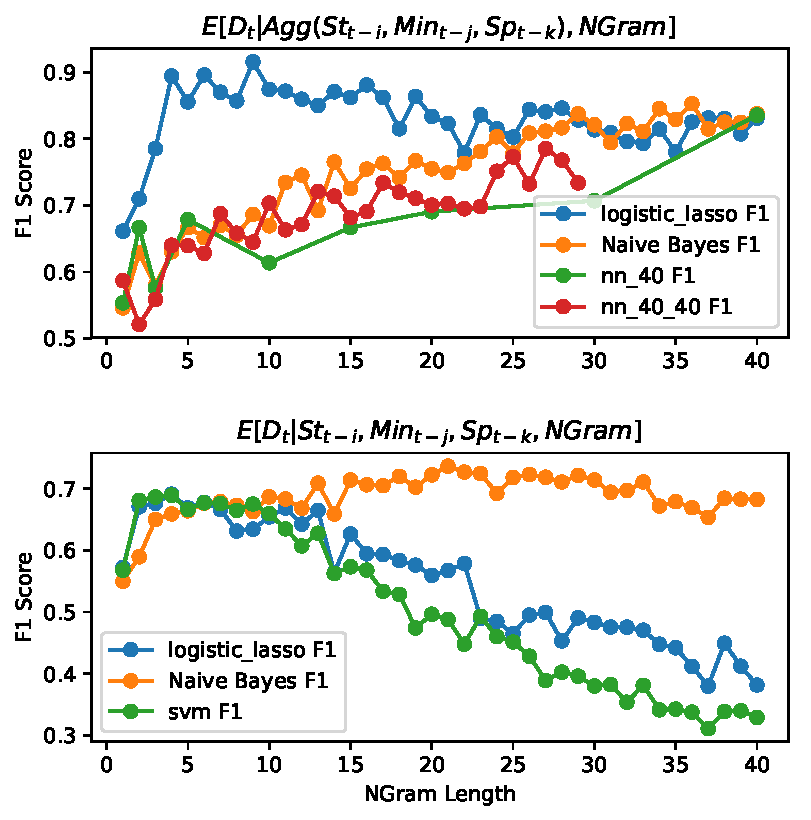
\includegraphics{./combined.pdf}
\end{figure}

\end{document}
